\chapter{Plugin Implementation}
\label{sec:PluginImplementation}
In this chapter we provide step-by-step instructions for implementing your own CrypTool 2 plugin. We shall assume that you have already retrieved the CrypTool 2 source code from the SVN repository, set up Visual Studio 2010 or Visual C\# 2010 Express to build CrypTool 2, and you have placed the plugin template in the right place.

\section{Downloading the example}
\label{sec:DownloadingTheExample}

We will use the \textbf{Caesar cipher} (also known as the \textbf{shift cipher}) as an example throughout this chapter. If you have not downloaded the entire CrypTool 2 source code as described in Section \ref{CheckingOutTheSources}, you can also get a copy of just the source code for the Caesar algorithm referenced throughout this guide from the following location:\\\\
\textit{username: anonymous\\
password:} (not required)\\
\url{https://www.cryptool.org/svn/CrypTool2/trunk/CrypPlugins/Caesar/}

\section{Creating a new project}
\label{sec:CreatingANewProject}

Open the CrypTool 2 solution, right click in the solution explorer on \textit{CrypPlugins} (or on the top solution item, if you're using Visual C\# Express) and select \textit{Add~$\rightarrow$ New Project}. In the dialog window, select \textit{Visual C\# $\rightarrow$ CrypTool 2.0 Plugin} as project template and enter a unique name for your new plugin project (such as \textit{Caesar} in our case). The \textbf{next step is crucial} to ensure that your plugin will compile and run correctly: select the subdirectory \texttt{CrypPlugins\textbackslash} as the location of your project (Figure~\ref{fig:vs_create_new_project}).

\begin{figure}[h!]
	\centering
		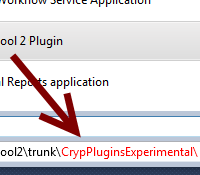
\includegraphics{figures/vs_create_new_project.png}
	\caption{Creating a new CrypTool 2 plugin project.}
	\label{fig:vs_create_new_project}
\end{figure}

As the project basics are already correctly set up in the template, you should now be able to compile the new plugin. First of all, rename the two files in the solution explorer to something more meaningful, for example \texttt{Caesar.cs} and \texttt{CaesarSettings.cs}.

\begin{figure}[h!]
	\centering
		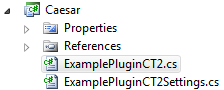
\includegraphics{figures/caesar_project.png}
	\caption{Items of a new plugin project.}
	\label{fig:caesar_project}
\end{figure}

\section{Adapting the plugin skeleton}
\label{AdaptingThePluginSkeleton}

If you look into the two C\# source files (Figure~\ref{fig:caesar_project}), you will notice a lot of comments marked with the keyword \texttt{HOWTO}. These are hints as to what you should change in order to adapt the plugin skeleton to your custom implementation. Most \texttt{HOWTO} hints are self-explanatory and thus we won't discuss them all in detail. For example, at the top of both source files, there is a hint to enter your name and affiliation in the license boilerplate:

\begin{lstlisting}
/* HOWTO: Change year, author name and organization.
   Copyright 2010 Your Name, University of Duckburg

\end{lstlisting}

After you have done this, remove the \texttt{HOWTO} hint:

\begin{lstlisting}
/*
   Copyright 2010 John Doe, University of Duisburg-Essen

\end{lstlisting}

\section{Defining the attributes of the Caesar class}
\label{sec:DefiningTheAttributesOfTheCaesarClass}

The next thing we will do in our example \textit{Caesar.cs} is define the attributes of our class. These attributes are used to provide necessary information for the CrypTool 2 environment. If they are not properly defined, your plugin won't show up in the application user interface, even if everything else is implemented correctly.

Attributes are used for declarative programming and provide metadata that can be added to the existing .NET metadata. CrypTool 2 provides a set of custom attributes that are used to mark the different parts of your plugin. These attributes should be defined right before the class declaration.
\clearpage

\subsection{The \protect\textit{[Author]} attribute}
\label{sec:TheAuthorAttribute}

The \textit{[Author]} attribute is optional, meaning that we are not required to define it. The attribute can be used to provide additional information about the plugin developer (or developers, as the case may be). This information will appear in the TaskPane, as for example in Appendix \ref{app:CaesarSettings}. We will define the attribute to demonstrate how it should look in case you want to use it in your plugin.

\begin{figure}[h!]
	\centering
		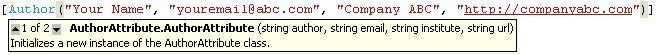
\includegraphics[width=.90\textwidth]{figures/attribute_author.jpg}
	\caption{The defintion for the \textit{[Author]} attribute.}
	\label{fig:attribute_author}
\end{figure}

As can be seen above, the author attribute takes four elements of type string. These elements are:

\begin{itemize}
	\item \textit{Author} --- the name of the plugin developer.
	\item \textit{Email} --- the email address of the plugin developer, should he or she wish to be available for contact.
	\item \textit{Institute} --- the organization, company or university with which the developer is affiliated.
	\item \textit{URL} --- the website of the developer or of his or her institution.
\end{itemize}

All of these elements are optional; the developer can choose what information will be published. Unused elements should be set to \texttt{null} or an empty string.

\subsection{The \protect\textit{[PluginInfo]} attribute}
\label{sec:ThePluginInfoAttribute}

The second attribute, \textit{[PluginInfo]}, provides necessary information about the plugin, and is therefore mandatory. The information defined in this attribute appears in the caption and tool tip window. The attribute is defined as follows:

\begin{figure}[h]
	\centering
		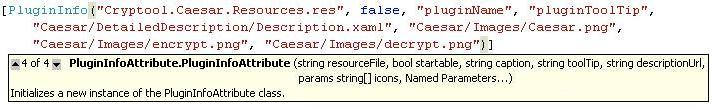
\includegraphics[width=1.00\textwidth]{figures/attribute_plugininfo.jpg}
	\caption{The defintion for the \textit{[PluginInfo]} attribute.}
	\label{fig:attribute_plugininfo}
\end{figure}

\noindent This attribute has the following parameters:

\begin{itemize}
	\item \textit{Resource File} --- the relative path of the associated resource file (if the plugin makes use of one). These files are used primarily to provide multilingual support for the plugin, although this is currently a work in progress. This element is optional.
	\item \textit{Startable} --- a flag that should be set to \texttt{true} only if the plugin is an input generator (i.e.\ if your plugin only has outputs and no inputs). In all other cases this should be set to \texttt{false}. This flag is important --- setting it incorrectly will result in unpredictable results. This element is mandatory.
	\item \textit{Caption} --- the name of the plugin, or, if using a resource file, the name of the field in the file with the caption data. This element is mandatory.
	\item \textit{ToolTip} --- a description of the plugin, or, if using a resource file, the name of the field in the resource file with the toolTip data. This element is optional.
	\item \textit{DescriptionURL} --- the local path of the description file (e.g.\ XAML file). This element is optional.
	\item \textit{Icons} --- an array of strings to define all the paths of the icons used in the plugin (i.e.\ the plugin icon described in Section \ref{sec:AddingAnIconToTheCaesarClass}). This element is mandatory.
\end{itemize}

\noindent Unused elements should be set to \texttt{null} or an empty string.

There are a few limitations and bugs that still exist in the \textit{[PluginInfo]} attribute that will be resolved in a future version. First, it is possible to use the plugin without setting a caption, although this is not recommended, and future versions of the plugin will fail to load without a caption. Second, a zero-length toolTip string currently causes the toolTip to appear as an empty box in the application. Third, the toolTip and description do not currently support internationalization and localization. Since the precise formulation and functionality of this attribute is still being developed, it is recommended to view other plugins for examples.

In our example, the \textit{resourceFile} parameter is set to \textit{Cryptool.Caesar.Resource.res}. This file will be used to store the label and caption text to support multilingualism.

The second parameter, \textit{startable}, should be set to \texttt{false}, because our encryption algorithm is not an input generator.

The next two parameters are necessary to define the plugin's name and description. Since we are using a resource file, we should place here the names of the resource fields that contain the caption and toolTip. (We could also just write simple text strings instead of using outsourced references.)

The \textit{DescriptionURL} element defines the location path of the description file. The parameter is composed in the format \textit{$<$assembly name$>$/$<$file name$>$} or, if you want to store your description files in a separate folder (as in our case), \textit{$<$assembly name$>$/$<$path$>$/$<$file name$>$}. The description file must be an XAML file. In our case, we shall create a folder named \textit{DetailedDescription} in which to store our XAML file with any necessary images. Our folder structure now looks as follows:

\begin{figure}[h!]
	\centering
		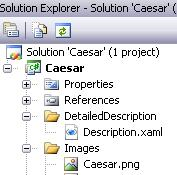
\includegraphics[width=.30\textwidth]{figures/detailed_description.jpg}
	\caption{The folder structure as seen in the Solution Explorer.}
	\label{fig:attribute_plugininfo_icon_path}
\end{figure}
\clearpage

Once a detailed description has been written in the XAML file, it can be accessed in the CrypTool~2 application by right-clicking on the plugin icon in the workspace and selecting \textit{Show description} \mbox{(Figure \ref{fig:xaml_description})}.

\begin{figure}[h!]
	\centering
		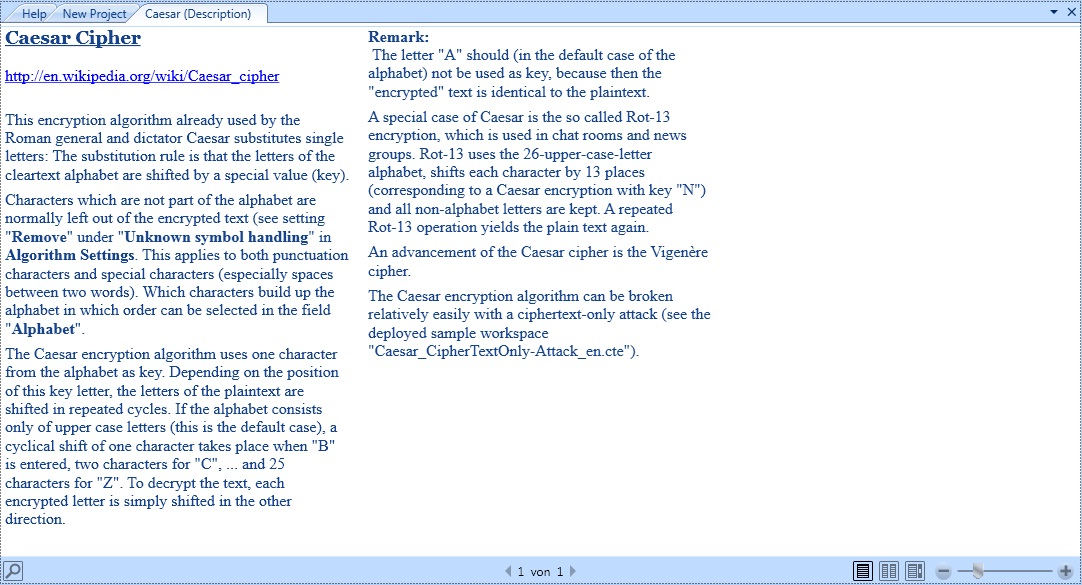
\includegraphics[width=1.00\textwidth]{figures/xaml_description.jpg}
	\caption{A detailed description provided through an XAML file.}
	\label{fig:xaml_description}
\end{figure}

The last parameter tells CrypTool 2 the names of the provided icons. This parameter is an array composed of strings in the format \textit{$<$assembly name$>$/$<$file name$>$} or \textit{$<$assembly name$>$/$<$path$>$/\linebreak $<$file~name$>$}.

The first and most important icon is the plugin icon, which will be shown in CrypTool 2 in the ribbon bar and navigation pane. Once the icon has been added to the project as described in Section~\ref{sec:AddingAnIconToTheCaesarClass}, we must accordingly tell CrypTool 2 where to find the icon. This can be seen above in Figure \ref{fig:attribute_plugininfo}.

If your plugin will use additional icons, you should define the paths to each of them by adding the path strings to the \textit{[PluginInfo]} attribute parameter list, each separated by a comma. We have added two further icons for the context menu in the CrypTool 2 workspace. (If you choose to add more icons, don't forget to add the icons to your solution.)

\subsection{Algorithm category and the \protect\textit{[EncryptionType]} attribute}
\label{sec:AlgorithmCategoryAndTheEncryptionTypeAttribute}

In the CrypTool 2 user interface plugins are grouped by their algorithm category, for example hash, encryption, and so on. To set the category, your plugin must inherit from a specific interface, like \textit{IHash} or \textit{IEncryption}. Some categories require the specification of a subcategory, which is entered as an attribute\footnote{The current category system is less than ideal and will be changed in future; see trac ticket \#50.}. In our example, Caesar inherits from \textit{IEncryption}.

\begin{lstlisting}
    [EncryptionType(EncryptionType.Classic)]
    public class Caesar : IEncryption
		{
\end{lstlisting}
\clearpage

The possible values of the \textit{[EncryptionType]} attribute are as follows:

\begin{itemize}
	\item \textit{Asymmetric} --- for asymmetrical encryption algorithms, such as RSA.
	\item \textit{SymmetricBlock} --- for block cipher algorithms, such as DES, AES and Twofish.
	\item \textit{SymmetricStream} --- for stream cipher algorithms, such as RC4, Rabbit and SEAL.
	\item \textit{Hybrid} --- for algorithms which are actually a combination of several algorithms, such as algorithms in which the data is encrypted symmetrically and the encryption key asymmetrically.
	\item \textit{Classic} --- for classical encryption or hash algorithms, such as Caesar or MD5.
\end{itemize}

\subsection{Importing CrypPluginBase namespaces}
\label{sec:ImportingCrypPluginBaseNamespaces}

Depending on which algorithm category you choose, you will need to import the corresponding namespace of \textit{CrypPluginBase}. To include the necessary namespaces in the class header, use the \texttt{using} statement followed by the name of the desired namespace. \textit{CrypPluginBase} provides the following namespaces:

\begin{itemize}
	\item \textit{Cryptool.PluginBase} --- contains interfaces such as \textit{IPlugin}, \textit{IHash}, and \textit{ISettings}, as well as attributes, enumerations, delegates and extensions.
	\item \textit{Cryptool.PluginBase.Analysis} --- contains interfaces for cryptanalysis plugins (such as \textit{Stream Comparator}).
	\item \textit{Cryptool.PluginBase.Control} --- contains global interfaces for the \textit{IControl} feature for defining custom controls.
	\item \textit{Cryptool.PluginBase.Cryptography} --- contains interfaces for encryption and hash algorithms such as AES, DES and MD5.
	\item \textit{Cryptool.PluginBase.Editor} --- contains interfaces for editors that can be implemented in CrypTool 2, such as the default editor.
	\item \textit{Cryptool.PluginBase.Generator} --- contains interfaces for generators, including the random input generator.
	\item \textit{Cryptool.PluginBase.IO} --- contains interfaces for input, output and the \textit{CryptoolStream}.
	\item \textit{Cryptool.PluginBase.Miscellaneous} --- contains assorted helper classes, including \textit{GuiLogMessage} and \textit{PropertyChanged}.
	\item \textit{Cryptool.PluginBase.Resources} --- used only by CrypWin and the editor; not necessary for plugin development.
	\item \textit{Cryptool.PluginBase.Tool} --- contains an interface for standalone tools in CrypTool~2 that are not run in a workspace editor.
	\item \textit{Cryptool.PluginBase.Validation} --- contains interfaces for validation methods, including regular expressions.
\end{itemize}

\noindent In our example, the Caesar algorithm necessitates the inclusion of the following namespaces:

\begin{itemize}
	\item \textit{Cryptool.PluginBase} --- to implement \textit{ISettings} in the CaesarSettings class.
	\item \textit{Cryptool.PluginBase.Cryptography} --- to implement \textit{IEncryption} in the Caesar class.
	\item \textit{Cryptool.PluginBase.IO} --- to use CryptoolStream for data input and output.
	\item \textit{Cryptool.PluginBase.Miscellaneous} --- to use the CrypTool event handler.
\end{itemize}

\section{Defining the private variables of the settings in the Caesar class}
\label{sec:DefiningThePrivateVariablesOfTheSettingsInTheCaesarClass}

The next step is to define some private variables that are needed for the settings, input, and output data. In our example, this will look like the following:

\begin{lstlisting}
	#region Private variables
	private CaesarSettings settings;
	private string inputString;
	private string outputString;
	private enum CaesarMode { encrypt, decrypt };
	private List<CryptoolStream> listCryptoolStreamsOut = new List<CryptoolStream>();
	#endregion
\end{lstlisting}

\ \\ % ugly but functional
If your algorithm deals with long strings of code, it is recommended to use the \textit{CryptoolStream} data type. This was designed for input and output between plugins and to handle large amounts of data. To use the native CrypTool stream type, include the namespace \textit{Cryptool.PluginBase.IO} with a \texttt{using} statement as explained in Section \ref{sec:ImportingCrypPluginBaseNamespaces}.

Our example makes use of the following private variables:

\begin{itemize}
	\item \texttt{CaesarSettings settings} --- required to implement the IPlugin interface properly.
	\item \texttt{string inputString} --- string from which to read the input data.
	\item \texttt{string outputString} --- string to which to save the output data.
	\item \texttt{enum CaesarMode} --- used to select either encryption or decryption.
	\item \texttt{List$<$CryptoolStream$>$ listCryptoolStreamsOut} --- a list of all streams created by the plugin, which helps to perform a clean dispose.
\end{itemize}

\subsection{Adding controls to the CaesarSettings class}
\label{sec:AddingControlsToTheCaesarSettingsClass}

The settings class contains the necessary information about controls, captions, descriptions, and default parameters (for key settings, alphabets, key length, type of action, etc.) to build the settings \textbf{TaskPane} in the CrypTool application. The settings class is used to populate the TaskPane in the CrypTool 2 application so that the user can modify the plugin settings at will. Therefore, we must implement some controls, such as buttons and text boxes, to allow for the necessary interaction. If you will be implementing an algorithm that does not have any user-defined settings (such as a hash function), then this class can be left mostly empty. In Appendix \ref{app:CaesarSettings} there is a full example of what a completed TaskPane and the corresponding source code for the existing Caesar plugin in CrypTool 2 looks like. You can also look at the source code of other CrypTool 2 plugins for examples of how to create the TaskPane backend.
\clearpage

\section{Adding an icon to the Caesar class}
\label{sec:AddingAnIconToTheCaesarClass}

Before we go back to the code of the Caesar class, we need to add a custom icon to our project to be shown in the CrypTool 2 \textbf{ribbon bar} and \textbf{navigation pane}. The template has a default icon set, so you don't need to create your own custom set.

The proper image size is 40x40 pixels, but since the image will be rescaled if necessary, any size is technically acceptable. Once you have saved your icon, you should add it directly to the project or to a subdirectory with it. In the project solution, create a new folder named \textit{Images}. This can be done by right-clicking on the project item (\textit{Caesar} in our example) and selecting \textit{Add $\rightarrow$ New Folder}. The icon can be added to this folder (or to the project directly, or to any other subdirectory) by right-clicking on the folder and selecting \textit{Add $\rightarrow$ Existing Item}.

\begin{figure}[h!]
	\centering
		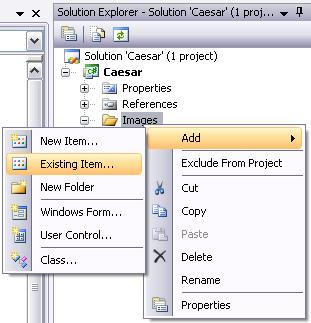
\includegraphics{figures/add_existing_item.jpg}
	\caption{Adding an existing item.}
	\label{fig:add_existing_item}
\end{figure}
\clearpage

A new window will then appear. Select \textit{Image Files} as the file type and select your newly-created icon for your plugin.

\begin{figure}[h!]
	\centering
		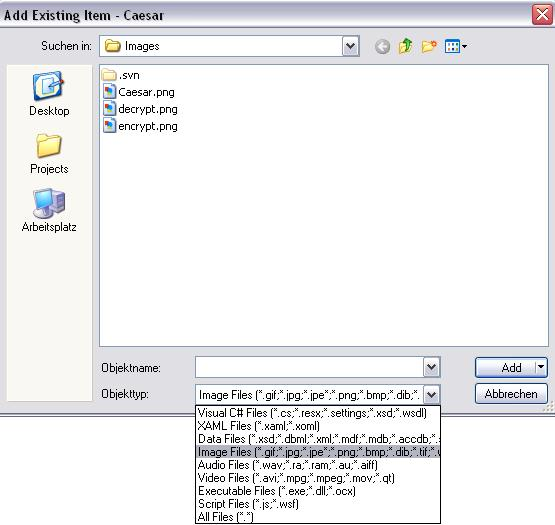
\includegraphics{figures/choose_icon.jpg}
	\caption{Selecting the image file.}
	\label{fig:choose_icon}
\end{figure}
\clearpage

Finally, we must set the icon as a \textit{Resource} to avoid including the icon as a separate file. Right-click on the icon and select \textit{Properties} as seen below.

\begin{figure}[h!]
	\centering
		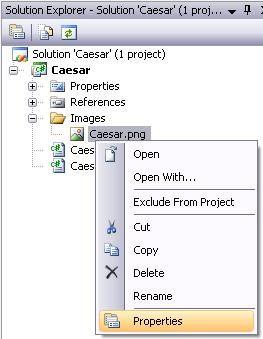
\includegraphics{figures/icon_properties.jpg}
	\caption{Selecting the image properties.}
	\label{fig:icon_properties}
\end{figure}

In the \textit{Properties} panel, set the \textit{Build Action} to \textit{Resource}.

\begin{figure}[h!]
	\centering
		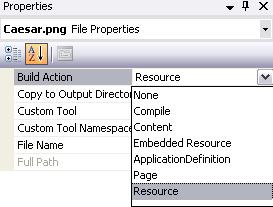
\includegraphics{figures/icon_build_action.jpg}
	\caption{Selecting the icon's build action.}
	\label{fig:icon_build_action}
\end{figure}
\clearpage

\section{Input and output dockpoints}
\label{sec:InputAndOutputDockpoints}

\subsection{The input/output attributes}
\label{sec:TheInputOutputAttributes}

Next we will define five properties, each with an appropriate attribute, to be used for input and output. Th attributes are necessary to tell CrypTool 2 whether the properties are used for input or output and to provide the plugin with external data.

The attribute that we will use for each proprerty is called \textit{[PropertyInfo]} and it consists of the following elements:

\begin{itemize}
	\item \textit{direction} --- defines whether this property is an input or output property, e.g.\ whether it reads input data or writes output data. The possible values are:
	\begin{itemize}
		\item \texttt{Direction.Input}
		\item \texttt{Direction.Output}
	\end{itemize}
	\item \textit{caption} --- the caption for the property displayed over the input or output arrow of the icon after it has been placed in the editor; ``Input stream'' in the example below:
	
\begin{figure}[h!]
	\centering
		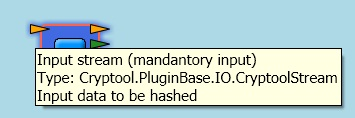
\includegraphics[width=.55\textwidth]{figures/property_caption.jpg}
	\caption{A possible property caption and toolTip.}
	\label{fig:property_caption}
\end{figure}

	\item \textit{toolTip} --- the toolTip for the property displayed over the input or output arrow of the icon after it has been placed in the editor; ``Input data to be hashed'' in the example above.
	\item \textit{descriptionUrl} --- currently not used; fill it with \texttt{null} or an empty string.
	\item \textit{mandatory} --- this flag determines whether an input must be attached by the user to use the plugin. If set to \texttt{true}, an input connection will be required or else the plugin will not be executed in the workflow chain. If set to \texttt{false}, connecting an input is optional. As this only applies to input properties, if the direction has been set to \texttt{Direction.Output}, this flag will be ignored.
	\item \textit{hasDefaultValue} --- if this flag is set to \texttt{true}, CrypTool 2 will assume that the property has a default input value that does not require user input.
	\item \textit{displayLevel} --- determines in which display levels your property will be shown in CrypTool~2. These are used to hide more advanced item from less-experienced users; a beginner using the corresponding display level will not see the properties marked as any other level, but a professional using the appropriate display level will have access to everything. These levels are as follows:
	
	\begin{itemize}
		\item \texttt{DisplayLevel.Beginner}
		\item \texttt{DisplayLevel.Experienced}
		\item \texttt{DisplayLevel.Expert}
		\item \texttt{DisplayLevel.Professional}
	\end{itemize}
	
	\item \textit{quickWatchFormat} --- determines how the content of the property will be shown in the quickwatch perspective. CrypTool 2 accepts the following quickwatch formats:
	
	\begin{itemize}
		\item \texttt{QuickWatchFormat.Base64}
		\item \texttt{QuickWatchFormat.Hex}
		\item \texttt{QuickWatchFormat.None}
		\item \texttt{QuickWatchFormat.Text}
	\end{itemize}

\begin{figure}[h]
	\centering
		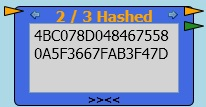
\includegraphics{figures/quick_watch.jpg}
	\caption{A quickwatch display in hexadecimal.}
	\label{fig:quick_watch}
\end{figure}
	
	\item \textit{quickWatchConversionMethod} --- this is used to indicate a conversion method; most plugins do not ned to convert their data and thus should use a \texttt{null} value here. The quickwatch function uses the default system encoding to display data, so if your data is in another format, such as UTF-16 or Windows-1250, you should provide here the name of a conversion method as string. The header for such a method should look something like the following:

\begin{lstlisting}
object YourMethodName(string PropertyNameToConvert)
\end{lstlisting}

\end{itemize}

\subsection{Defining the input/output properties}
\label{sec:DefiningTheInputOutputProperties}

The first of the five properties that we will define is \textit{InputString}. This is used to provide our plugin with the data to be encrypted or decrypted:

\begin{lstlisting}
[PropertyInfo(Direction.InputData, "Text input", "Input a string to be processed by the Caesar cipher", "", true, false, DisplayLevel.Beginner, QuickWatchFormat.Text, null)]
public string InputString
{
	get { return this.inputString; }
	set
  {
		if (value != inputString)
		{
			this.inputString = value;
			OnPropertyChanged("InputString");
		}
	}
}
\end{lstlisting}

\ \\
In the get method we simply return the value of the input data. The set method checks if the input value has changed, and, if so, sets the new input data and announces the change to the CrypTool 2 environment by calling the function \textit{OnPropertyChanged(\textit{$<$Property name$>$})}. This step is necessary for input properties to update the quickwatch view. The output data property (which handles the input data after it has been encrypted or decrypted) will in our example look as follows:

%\textit{\small Note 1: It is currently not possible to read directly from the input data stream without creating an intermediate CryptoolStream.\\\\
%\small Note 2: The naming may be confusing. The new CryptoolStream is not an output stream, but it is added to the list of output streams to enable a clean dispose afterwards. See chapter 9 below.\\\\}

\begin{lstlisting}
[PropertyInfo(Direction.OutputData, "Text output", "The string after processing with the Caesar cipher", "", false, false, DisplayLevel.Beginner, QuickWatchFormat.Text, null)]
public string OutputString
{
	get { return this.outputString; }
	set
	{
		outputString = value;
		OnPropertyChanged("OutputString");
	}
}
\end{lstlisting}

\ \\
\indent CrypTool 2 does not require implementing set methods for output properties, as they will never be called from outside the plugin. Nevertheless, in our example the plugin itself accesses the property, and therefore we have chosen to implement the set method.

You can provide additional output data types if you so desire. In our example, we will also offer output data of type \textit{CryptoolStream}, input data for external alphabets, and input data for the shift value of our Caesar algorithm. Note that for the first of these, the set method is not implemented since it will never be called. We shall define these properties as follows:

\begin{lstlisting}
[PropertyInfo(Direction.OutputData, "CryptoolStream output", "The raw CryptoolStream data after processing with the Caesar cipher", "", false, false, DisplayLevel.Beginner, QuickWatchFormat.Text, null)]
public CryptoolStream OutputData
{
	get
	{
		if (outputString != null)
		{
			CryptoolStream cs = new CryptoolStream();
			listCryptoolStreamsOut.Add(cs);
			cs.OpenRead(Encoding.Default.GetBytes(outputString.ToCharArray()));
			return cs;
		}
		else
		{
			return null;
		}
	}
	set { }
}

[PropertyInfo(Direction.InputData, "External alphabet input", "Input a string containing the alphabet to be used by Caesar.\nIf no alphabet is provided for this input, the internal default alphabet will be used.", "", false, false, DisplayLevel.Expert, QuickWatchFormat.Text, null)]
public string InputAlphabet
{
	get { return ((CaesarSettings)this.settings).AlphabetSymbols; }
	set
	{
		if (value != null && value != settings.AlphabetSymbols)
		{
			((CaesarSettings)this.settings).AlphabetSymbols = value;
			OnPropertyChanged("InputAlphabet");
		}
	}
}

[PropertyInfo(Direction.InputData, "Shift value (integer)", "This is the same setting as the shift value in the Settings pane but as dynamic input.", "", false, false, DisplayLevel.Expert, QuickWatchFormat.Text, null)]
public int ShiftKey
{
	get { return settings.ShiftKey; }
	set
	{
		if (value != settings.ShiftKey)
		{
			settings.ShiftKey = value;
		}
	}
}
\end{lstlisting}

\section{Implementing the actual algorithm}
\label{sec:ImplementingTheActualAlgorithm}

Algorithmic processing should be done in the \textit{Execute()} function. The actual functionality of your algorithm, as well as the structure thereof, is up to you. Below is our implementation of the Caesar algorithmic processing and the \textit{Execute()} function:

\begin{lstlisting}
private void ProcessCaesar(CaesarMode mode)
{
	CaesarSettings cfg = (CaesarSettings)this.settings;
	StringBuilder output = new StringBuilder("");
	string alphabet = cfg.AlphabetSymbols;

	// If we are working in case-insensitive mode, we will use only
	// capital letters, hence we must transform the whole alphabet
	// to uppercase.
	if (!cfg.CaseSensitiveAlphabet)
	{
		alphabet = cfg.AlphabetSymbols.ToUpper();
	}

	if (inputString != null)
	{
		for (int i = 0; i < inputString.Length; i++)
		{
			// Get the plaintext char currently being processed.
			char currentchar = inputString[i];

			// Store whether it is upper case (otherwise lowercase is assumed).
			bool uppercase = char.IsUpper(currentchar);

			// Get the position of the plaintext character in the alphabet.
			int ppos = 0;
			if (cfg.CaseSensitiveAlphabet)
			{
				ppos = alphabet.IndexOf(currentchar);
			}
			else
			{
				ppos = alphabet.IndexOf(char.ToUpper(currentchar));
			}

			if (ppos >= 0)
			{
				// We found the plaintext character in the alphabet,
				// hence we will commence shifting.
				int cpos = 0;
				switch (mode)
				{
					case CaesarMode.encrypt:
						cpos = (ppos + cfg.ShiftKey) % alphabet.Length;
						break;
					case CaesarMode.decrypt:
						cpos = (ppos - cfg.ShiftKey + alphabet.Length) % alphabet.Length;
						break;
				}

				// We have the position of the ciphertext character,
				// hence just output it in the correct case.
				if (cfg.CaseSensitiveAlphabet)
				{
					output.Append(alphabet[cpos]);
				}
				else
				{
					if (uppercase)
					{
						output.Append(char.ToUpper(alphabet[cpos]));
					}
					else
					{
						output.Append(char.ToLower(alphabet[cpos]));
					}
				}
			}
			else
			{
				// The plaintext character was not found in the alphabet,
				// hence proceed with handling unknown characters.
				switch ((CaesarSettings.UnknownSymbolHandlingMode)cfg.UnknownSymbolHandling)
				{
					case CaesarSettings.UnknownSymbolHandlingMode.Ignore:
						output.Append(inputString[i]);
						break;
					case CaesarSettings.UnknownSymbolHandlingMode.Replace:
						output.Append('?');
						break;
				}
			}

			// Show the progress.
			ProgressChanged(i, inputString.Length - 1);
		}
		outputString = output.ToString();
		OnPropertyChanged("OutputString");
		OnPropertyChanged("OutputData");
	}
}

public void Execute()
{
	switch (settings.Action)
	{
		case 0:
			GuiLogMessage("Encrypting", NotificationLevel.Debug);
			ProcessCaesar(CaesarMode.encrypt);
			break;
		case 1:
			GuiLogMessage("Decrypting", NotificationLevel.Debug);
			ProcessCaesar(CaesarMode.decrypt);
			break;
		default:
    	break;
	}
}
\end{lstlisting}

It is important to make sure that all changes to the output properties will be announced to the CrypTool 2 environment. In our example this happens by calling the set method of \textit{OutputData}, which in turn calls \textit{OnPropertyChanged} to indicate that both output properties \textit{OutputData} and \textit{OutputDataStream} have changed. Instead of calling the property's set method you could instead call \textit{OnPropertyChanged} directly within the \textit{Execute()} method.

\subsection{Sending messages to the CrypTool 2 core}
\label{sec:SendingMessagesToTheCrypTool2Core}

The CrypTool 2 API provides three methods to send messages from the plugin to the CrypTool 2 core. \textit{GuiLogMessage} is used to send messages to the CrypTool 2 status bar. This method is a nice mechanism to inform the user as to what your plugin is currently doing. \textit{OnPropertyChanged} is used to inform the core application of changes to any data output properties. This is necessary for a correct plugin execution. \textit{ProgressChanged} is used to visualize the progress of the algorithm as a bar.

\begin{figure}[h]
	\centering
		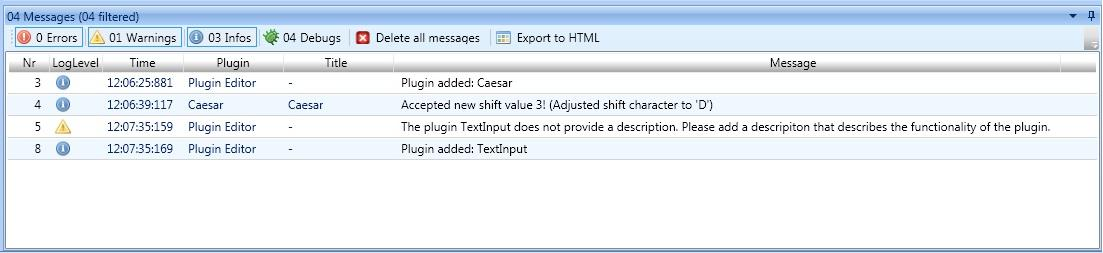
\includegraphics[width=1.00\textwidth]{figures/status_bar.jpg}
	\caption{An example status bar.}
	\label{fig:status_bar}
\end{figure}

The \textit{GuiLogMessage} method takes two parameters:

\begin{itemize}
	\item \textit{Message} --- the text to be shown in the status bar.
	\item \textit{NotificationLevel} --- the type of message, that is, its alert level:
	\begin{itemize}
		\item \texttt{NotificationLevel.Error}
		\item \texttt{NotificationLevel.Warning}
		\item \texttt{NotificationLevel.Info}
		\item \texttt{NotificationLevel.Debug}
	\end{itemize}
\end{itemize}

\subsection{Performing a clean dispose}
\label{sec:PerformingACleanDispose}

Be sure you have closed and cleaned all your streams after execution before CrypTool 2 decides to dispose the plugin instance. There has been some misunderstanding about the meaning of \textit{Dispose()}. Dispose will be called ultimately before object destruction. After disposal, the object will be in an undefined state.

\begin{lstlisting}
public void Dispose()
{
	foreach(CryptoolStream stream in listCryptoolStreamsOut)
	{
		stream.Close();
	}
	listCryptoolStreamsOut.Clear();
}
\end{lstlisting}

\section{Drawing the workflow of your plugin}
\label{DrawingTheWorkfloweOfYourPlugin}

Each plugin should have an associated workflow file to show the algorithm in action in CrypTool 2. These workflow files are saved with the special \textit{.cte} file extension. You can view the example files from other plugins by opening any of the files in the \texttt{ProjectSamples\textbackslash} folder with CrypTool 2. Below is a sample workflow for our Caesar example:

\begin{figure}[h]
	\centering
		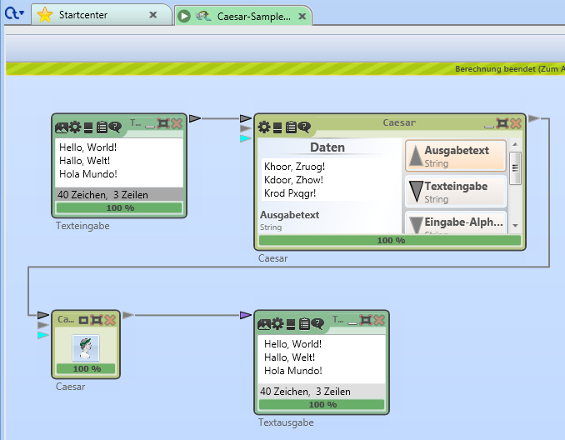
\includegraphics{figures/sample.jpg}
	\caption{A sample workflow diagram for the Caesar algorithm.}
	\label{fig:sample}
\end{figure}

As your last step of development, once your plugin runs smoothly, you should also create one of these sample workflow files for your plugin. Such a file can be automatically created by simply saving a CrypTool 2 workspace project featuring your plugin. You should store the workflow file in the \texttt{ProjectSamples\textbackslash} folder and make sure to commit the file to the SVN repository (see Section \ref{CommitingYourChanges}).